Para el propósito de predecir y comprender con precisión el comportamiento del usuario, se desarrolló e implementó un modelo de clasificación avanzado. Este modelo se basó en el análisis de un conjunto de datos detallado y complejo, que incluía múltiples variables y patrones de interacción de los usuarios. La finalidad de este modelo es no solo prever las acciones futuras de los usuarios, sino también desentrañar las dinámicas subyacentes y las tendencias en su comportamiento. La implementación de este modelo de clasificación juega un papel crucial en la generación de insights valiosos y en la toma de decisiones informadas basadas en el análisis de datos.

\subsection{Preprocesamiento y Preparación de Datos}

El proceso de preparación de los datos comenzó con la importación de la información desde un archivo CSV, seguida de una meticulosa etapa de limpieza para asegurar la integridad y relevancia de los datos. Durante esta etapa, se realizaron filtros específicos en la columna “método” y se descartaron registros en los que la columna “canal” estaba vacía. Esta selección tenía como objetivo eliminar elementos irrelevantes o incompletos que podrían distorsionar los resultados del análisis. Adicionalmente, se llevó a cabo la conversión de las marcas temporales al formato UTC, una medida crucial para lograr una estandarización homogénea a lo largo de todo el conjunto de datos.

El preprocesamiento es un paso crítico para garantizar que los datos estén limpios, completos y adecuadamente preparados para el modelado. Esta fase incluyó la eliminación o corrección de valores atípicos, el manejo de valores faltantes y la confirmación de la consistencia de los datos. La decisión de filtrar métodos específicos y eliminar registros con campos de canales vacíos se tomó con el fin de conservar únicamente aquellos datos que aportan valor significativo al análisis. La estandarización de las marcas temporales a UTC es fundamental para asegurar la precisión en el análisis temporal, permitiendo comparaciones efectivas de eventos a través de diferentes zonas horarias.
\subsection{Ordenamiento y Etiquetado}
En la fase de preparación de los datos para nuestro modelo de clasificación secuencial, se implementó un proceso de ordenamiento cronológico por usuario y fecha de evento, crucial para preservar la secuencia de acciones de cada usuario. Este ordenamiento se realizó agrupando las acciones en el conjunto de datos por la columna \textquotedblleft rut\_cliente\textquotedblright y luego ordenándolas dentro de cada grupo según la \textquotedblleft fecha\_evento\textquotedblright. Este procedimiento asegura que se mantenga la secuencia temporal de las actividades, una práctica esencial para modelos que requieren comprender y aprender de las transiciones entre diferentes acciones o estados de un usuario.

Posteriormente, procedimos a la generación de etiquetas para el aprendizaje supervisado. Excluyendo la última acción de cada secuencia o sesión, cada acción fue etiquetada con la acción subsiguiente empleando el método \textquotedblleft .shift(-1)\textquotedblright en el DataFrame agrupado. Esta técnica desplaza las acciones hacia arriba, permitiendo así que cada acción se alinee con su sucesora inmediata. Las acciones siguientes se utilizaron como etiquetas para las acciones precedentes, y para las últimas acciones de las secuencias, donde no hay una acción sucesiva, se asignó una etiqueta específica como \textquotedblleft final\_del\_recorrido\textquotedblright para indicar el fin de la sesión.

Este enfoque es vital para el entrenamiento de modelos de aprendizaje supervisado, particularmente en el contexto de modelos secuenciales como las Redes Neuronales Recurrentes (RNN) o las de Memoria a Corto y Largo Plazo (LSTM). Proporciona al modelo los \textquotedblleft objetivos\textquotedblright a predecir, basándose en el contexto de las acciones previas. Con este proceso, cada acción en el conjunto de datos se asocia con una etiqueta que representa la acción futura inmediata, creando así un conjunto de datos listo para el entrenamiento de un modelo predictivo capaz de anticipar el comportamiento futuro del usuario a partir de su historial de interacciones.

\subsection{Identificación de Sesiones}

Para obtener una comprensión más profunda de las interacciones de los usuarios con el sistema, procedimos a segmentar el flujo continuo de datos en lo que denominamos sesiones discretas. En este contexto, una sesión se define como un conjunto de eventos consecutivos llevados a cabo por un usuario, los cuales están limitados por períodos de inactividad que no exceden un umbral de tiempo predeterminado. Este criterio de segmentación nos permite identificar y analizar las secuencias de acciones realizadas por los usuarios, considerando como límite de una sesión la presencia de una pausa significativa en su actividad. Esta definición de sesión es crucial para el análisis detallado del comportamiento de los usuarios, ya que facilita la identificación de patrones y tendencias dentro de las interacciones individuales con el sistema.

\subsubsection{Cálculo de Diferencias de Tiempo} 
El proceso de análisis se inició con el cálculo de los intervalos de tiempo entre eventos consecutivos para cada usuario. Esta tarea se llevó a cabo aplicando el método .diff() a la columna de marcas temporales en nuestro conjunto de datos. Para asegurar la precisión de esta operación, la columna de marcas temporales fue previamente ordenada por usuario y por la fecha de cada evento. Como resultado de la aplicación de este método, se generó una nueva columna en el conjunto de datos. Esta columna adicional representa el tiempo transcurrido entre cada acción registrada y la acción subsiguiente, proporcionando así una medida cuantitativa del intervalo temporal entre eventos sucesivos. Esta información es crucial para identificar patrones de comportamiento y para la determinación de sesiones dentro del flujo de interacción del usuario.

\subsubsection{Definición de un Umbral de Tiempo} 
Para la identificación de nuevas sesiones en nuestro análisis, se estableció un umbral temporal específico. La definición de este umbral se basó en un estudio detallado del patrón de uso característico del sitio web. Se determinó que un período de inactividad superior a 30 minutos es indicativo del final de una sesión de usuario. Esta decisión se fundamenta en la observación de que lapsos prolongados sin actividad tienden a representar una pausa natural o conclusión en la interacción del usuario con el sitio. La implementación de este umbral temporal es esencial para segmentar el conjunto de datos de manera precisa, permitiendo así una evaluación más estructurada y coherente de las sesiones de usuario para fines de análisis y modelación predictiva.

\subsubsection{Identificación de Nuevas Sesiones}
Mediante la comparación de las diferencias temporales con un umbral preestablecido, fue posible identificar el comienzo de nuevas sesiones en el conjunto de datos. En este contexto, un valor que excede el umbral establecido en la columna de diferencias de tiempo es indicativo de que la acción correspondiente marca el inicio de una nueva sesión. Esta metodología se basa en la premisa de que intervalos de tiempo sustancialmente largos entre acciones consecutivas son representativos de una pausa en la interacción del usuario, y por lo tanto, señalan el comienzo de una nueva sesión de actividad. Esta técnica es esencial para segmentar adecuadamente el conjunto de datos en sesiones individuales, lo cual es fundamental para el análisis detallado y la modelación predictiva del comportamiento de los usuarios en secuencias temporales.

\subsubsection{Asignación de Identificadores de Sesión} 
Para identificar claramente las nuevas sesiones en nuestro conjunto de datos, se llevó a cabo una transformación de los valores booleanos, obtenidos como resultado de la comparación con el umbral establecido, en un identificador numérico acumulativo. Este proceso se implementó mediante el uso del método .cumsum(), el cual incrementa automáticamente el identificador cada vez que se detecta el inicio de una nueva sesión. De este modo, se asigna un número único y secuencial a cada sesión para cada usuario, facilitando así la distinción y el seguimiento de las distintas sesiones en el análisis posterior. Este enfoque asegura una organización coherente y una identificación precisa de las sesiones individuales dentro del conjunto de datos, lo cual es crucial para el análisis detallado y la modelación predictiva del comportamiento de los usuarios.

El código que se utilizó para llevar a cabo este proceso esencial de estructuración de datos se presenta a continuación. Este fragmento de código desempeña un papel crucial en la organización de los datos, asegurando que reflejen adecuadamente los períodos de interacción activa de los usuarios con el sistema. La implementación correcta de este código es fundamental para la preparación de los datos, facilitando un análisis detallado y una modelación predictiva eficaz del comportamiento futuro de los usuarios. El siguiente código detalla cómo se efectuó esta transformación y estructuración de los datos:

\begin{figure}[H]
    \begin{minipage}[t]{0.9\textwidth}
        \caption{Código indentificación de sesiones}
        \label{identificación_sesiones}        
    \end{minipage}

    \vspace{10pt}

    \begin{minipage}[b]{1\textwidth}
        \centering
        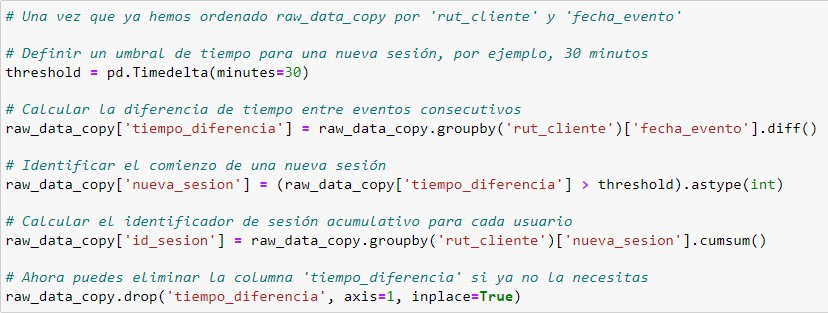
\includegraphics[width=\textwidth]{img/Código identificación sesiones.jpg}        
    \end{minipage}

    \begin{minipage}[t]{0.9\textwidth}
        Fuente: Elaboración propia.
    \end{minipage}
\end{figure}

Este método de estructuración de los datos fue fundamental para capturar con exactitud los períodos de interacción activa de los usuarios con el sistema. Al reflejar de manera precisa estas secuencias de interacción, se estableció una base sólida y fiable para el análisis detallado y la modelación predictiva del comportamiento futuro de los usuarios. Este enfoque es esencial en el aprendizaje automático, ya que proporciona el contexto y la profundidad necesarios para que el modelo pueda identificar patrones significativos y tendencias en el comportamiento de los usuarios, lo cual es crucial para realizar predicciones precisas y significativas sobre sus acciones futuras.

\subsection{Codificación de Categorías}

En el campo del aprendizaje automático, es frecuente el manejo de datos categóricos, es decir, información que no se presenta en forma numérica. Un ejemplo claro son los nombres de métodos y canales en nuestro conjunto de datos. Para facilitar el procesamiento de estos datos por parte de un modelo de clasificación, es imperativo convertir estas categorías textuales a un formato numérico que el modelo pueda interpretar y manejar de manera eficiente. Este proceso de transformación se denomina codificación de categorías. La realización de esta codificación es esencial para que el modelo pueda analizar adecuadamente los datos y generar predicciones precisas. A continuación, detallamos cómo se implementó este proceso de codificación en nuestros datos:

\subsubsection{Mapeo de Categorías a Números:}

\begin{itemize}
    \item En el proceso de preparación de nuestros datos, se establecieron dos diccionarios distintos: uno dedicado a los \textbf{métodos} y otro a los \textbf{canales}. Esta separación asegura una organización clara y específica, permitiendo que cada tipo de información sea codificado y manejado de manera independiente. La creación de un diccionario específico para los métodos y otro para los canales facilita el mapeo preciso de estas categorías a valores numéricos, lo cual es esencial para el procesamiento posterior y el análisis en el contexto del modelo de aprendizaje automático.
    \item Cada diccionario en nuestro enfoque de procesamiento de datos está diseñado para asignar de manera unívoca una categoría textual a un número entero distinto. Esta correspondencia uno a uno entre las categorías textuales y los valores numéricos enteros es fundamental para la conversión eficiente de datos cualitativos en una forma cuantitativa que pueda ser procesada y analizada por el modelo de aprendizaje automático. Este mapeo asegura que cada categoría textual, representando una característica específica o una acción dentro del conjunto de datos, tenga una representación numérica única, lo cual es esencial para la integridad y la coherencia del proceso de modelado.
    \item Como ilustración, en nuestro proceso de mapeo, el método \textbf{login()} se asigna al valor numérico 1, mientras que el método \textbf{getAccounts()} se asocia con el número 2. Este patrón de asignación numérica se repite de manera similar para los demás métodos en el conjunto de datos. Estos mapeos transforman las funciones y operaciones del usuario, originalmente expresadas en forma textual o de código, en una serie de valores numéricos discretos. Esta conversión es esencial para permitir el procesamiento computacional y el análisis cuantitativo en las etapas de modelado y entrenamiento del sistema de aprendizaje automático.
\end{itemize}

\subsubsection{Aplicación de la Codificación:}

\begin{itemize}
    \item En el proceso de preparación de nuestros datos, empleamos diccionarios específicos para convertir todas las instancias de métodos y canales en nuestro DataFrame a formatos numéricos. Esta transformación implicó reemplazar cada método y canal presente en el conjunto de datos por su respectivo valor numérico, tal como se define en los diccionarios de mapeo. Este enfoque asegura una representación uniforme y cuantificable de estas variables, facilitando su manipulación y análisis por parte del modelo de aprendizaje automático. La conversión a valores numéricos es esencial para la eficacia del procesamiento de datos y para la realización de operaciones matemáticas y estadísticas relevantes en las etapas subsiguientes del modelado.
\end{itemize}

\subsubsection{Beneficios de la Codificación}

\begin{itemize}
    \item La transformación de los datos a un formato numérico es un aspecto crítico en el campo del aprendizaje automático, dado que los modelos en esta área operan de manera más eficiente con variables numéricas. Estas variables permiten la aplicación de operaciones matemáticas y técnicas estadísticas durante el proceso de entrenamiento del modelo. La representación numérica facilita el manejo y procesamiento de los datos, permitiendo que el modelo realice cálculos complejos, optimice patrones y extraiga insights significativos. Esta capacidad es fundamental para el desarrollo de modelos que pueden aprender, adaptarse y realizar predicciones precisas basadas en los datos proporcionados.
    \item La codificación de categorías facilita la implementación de algoritmos de incrustación (embedding), los cuales son fundamentales en el análisis avanzado de datos. Estos algoritmos de embedding tienen la capacidad de capturar y representar información sobre las categorías en un espacio de características multidimensionales, proporcionando una riqueza y una profundidad mayor que la que se obtendría mediante una simple representación numérica entera. Este enfoque permite al modelo discernir y aprender de las sutilezas y relaciones complejas inherentes a las categorías, resultando en una representación de datos más rica y matizada que es esencial para mejorar la precisión y efectividad de las predicciones del modelo.
\end{itemize}

A continuación se presenta el fragmento de código implementado para llevar a cabo la codificación de categorías. Este código es un componente crucial en el proceso de preparación de los datos, ya que transforma las categorías de métodos y canales en un formato que puede ser procesado eficazmente por nuestro modelo de clasificación secuencial. La codificación adecuada es esencial para permitir que el modelo interprete y utilice esta información categórica de manera efectiva en sus procesos de aprendizaje y predicción. El siguiente código detalla cómo se realizó esta transformación:

\begin{figure}[H]
    \begin{minipage}[t]{0.9\textwidth}
        \caption{Código codificación de categorías}
        \label{codificación_categorias}        
    \end{minipage}

    \vspace{10pt}

    \begin{minipage}[b]{1\textwidth}
        \centering
        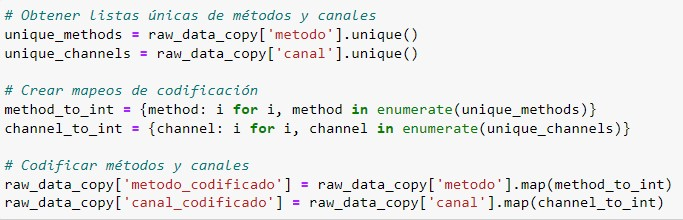
\includegraphics[width=\textwidth]{img/Código codificación categorias.jpg}        
    \end{minipage}

    \begin{minipage}[t]{0.9\textwidth}
        Fuente: Elaboración propia.
    \end{minipage}
\end{figure}

La codificación de categorías representa una etapa preparatoria crítica en el proceso de preparación de datos para nuestro modelo de clasificación secuencial. Esta fase de codificación es fundamental para que el modelo pueda interpretar eficazmente los patrones presentes en los métodos y canales utilizados por los usuarios. Al convertir estas categorías en un formato estructurado y legible por la máquina, se mejora considerablemente la habilidad del modelo para analizar y comprender la secuencia de acciones del usuario. Esto, a su vez, incrementa significativamente la precisión del modelo en la realización de predicciones informadas sobre las posibles acciones futuras que el usuario podría emprender. Este paso es, por lo tanto, esencial para asegurar que el modelo no solo capture la secuencia de eventos, sino que también derive insights relevantes y significativos a partir de ellos.

\subsection{Construcción de Secuencias}

La construcción de secuencias constituye un paso fundamental en la preparación de datos para el modelado en contextos de series temporales o secuenciales, como es el caso de nuestro modelo de clasificación. Este proceso implica la organización y estructuración meticulosa de los datos para que reflejen con precisión las secuencias naturales de interacciones de los usuarios. Tal organización es clave para preservar la integridad temporal y la secuencialidad inherente a los patrones de comportamiento de los usuarios. A continuación, detallamos el enfoque y los pasos específicos empleados para llevar a cabo esta tarea esencial:

\subsubsection{Agrupación de Eventos en Secuencias:}

\begin{itemize}
    \item Una vez completada la codificación de los métodos y canales, cada acción individual del usuario queda representada por un par de números codificados. El paso subsiguiente en el proceso de modelado de datos implica la agrupación de estas acciones codificadas en secuencias. Estas secuencias están diseñadas para representar de manera integral la trayectoria completa de la interacción del usuario durante una sesión específica. Este enfoque permite capturar la secuencia y el flujo de las actividades del usuario, proporcionando así un contexto detallado y estructurado que es esencial para el análisis posterior y el entrenamiento del modelo de aprendizaje automático.
    \item Cada secuencia en nuestro modelo se forma a partir de pares de métodos y canales codificados, y se construye específicamente para cada usuario y para cada sesión que se haya identificado previamente. Para lograr esto, los datos se organizan mediante un proceso de agrupación por usuario y sesión. Posteriormente, dentro de cada grupo, se listan las acciones codificadas siguiendo un orden cronológico. Este enfoque permite que cada secuencia refleje con precisión la secuencia temporal de eventos para un usuario en una sesión determinada, asegurando así que el modelo pueda capturar y aprender de la dinámica y el flujo de las interacciones del usuario.
\end{itemize}

\subsubsection{Preparación para el Modelo de Red Neuronal:}

\begin{itemize}
    \item Las secuencias numéricas generadas constituyen el insumo principal para la alimentación de la red neuronal. En el ámbito de las Redes Neuronales Recurrentes (RNN), incluyendo las de tipo Long Short-Term Memory (LSTM), estas secuencias son fundamentales para el modelo, ya que le permiten reconocer y aprender patrones temporales y dependencias entre eventos consecutivos. La capacidad de las LSTM y otras RNN de procesar estas secuencias numéricas les confiere la habilidad única de capturar y analizar la dinámica temporal inherente a los datos, lo cual es esencial para la predicción precisa y el análisis de series temporales.
\end{itemize}

\subsubsection{Estructura de Datos de Secuencias:}

\begin{itemize}
    \item Desde la perspectiva de la estructura de datos, las secuencias se organizan comúnmente como listas de listas (o arrays de arrays), en las cuales cada sublista representa una secuencia completa correspondiente a un usuario. Esta forma de organización de datos es idónea para modelar secuencias, ya que permite encapsular una serie de eventos o acciones consecutivas de cada usuario de manera estructurada y coherente. En este esquema, cada sublista contiene los elementos que componen una secuencia individual, reflejando la cronología y la progresión de las acciones del usuario. Este formato es ampliamente utilizado en el procesamiento de secuencias temporales, proporcionando una representación clara y eficiente que facilita el análisis y el aprendizaje automático.
\end{itemize}

A continuación, se presenta el fragmento de código utilizado para la construcción de secuencias en nuestro modelo. Este código es esencial para transformar los datos crudos en una forma estructurada que el modelo pueda procesar eficientemente. La construcción de secuencias es un paso crítico en la preparación de datos para modelado predictivo, ya que permite que el modelo aprenda a identificar y seguir patrones de comportamiento a lo largo del tiempo. El siguiente código ilustra cómo se lleva a cabo esta transformación:

\begin{figure}[H]
    \begin{minipage}[t]{0.9\textwidth}
        \caption{Código construcción de secuencias}
        \label{construcción_secuencias}        
    \end{minipage}

    \vspace{10pt}

    \begin{minipage}[b]{1\textwidth}
        \centering
        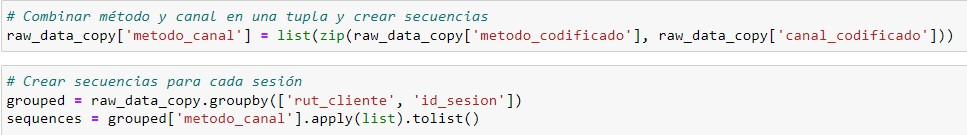
\includegraphics[width=\textwidth]{img/Código construcción de secuencias.jpg}        
    \end{minipage}

    \begin{minipage}[t]{0.9\textwidth}
        Fuente: Elaboración propia.
    \end{minipage}
\end{figure}

\subsubsection{Significado para el Modelado Predictivo:}

\begin{itemize}
    \item Las secuencias desempeñan un rol crucial en el ámbito del modelado predictivo, ya que suministran el contexto integral necesario para que el modelo realice predicciones basadas en información relevante. Por ejemplo, al analizar la secuencia de acciones realizadas previamente por un usuario, es posible inferir patrones conductuales que indican cuál podría ser la próxima acción. Un caso ilustrativo sería una secuencia donde el usuario realiza varias consultas de información, lo que podría llevar al modelo a predecir que la acción subsiguiente más probable sería "cerrar sesión". Este tipo de análisis secuencial permite al modelo capturar y aprender de las tendencias y patrones en el comportamiento del usuario, facilitando así predicciones más precisas y contextualizadas.
\end{itemize}

\subsubsection{Alineación con Objetivos de Predicción:}

\begin{itemize}
    \item Además, las secuencias generadas se encuentran alineadas con las etiquetas que se definieron en la fase de etiquetado. En este proceso, cada acción dentro de una secuencia, con la excepción de la última, se asocia con una etiqueta correspondiente que indica la acción subsiguiente. Esta metodología es esencial para el entrenamiento del modelo, ya que facilita la tarea de predecir la próxima acción basándose en la secuencia de acciones anteriores. La correcta alineación de secuencias con sus etiquetas correspondientes es crucial, ya que proporciona al modelo el contexto necesario para aprender a anticipar las acciones futuras de manera precisa, basándose en patrones de comportamiento observados previamente.
\end{itemize}

La construcción de secuencias es un proceso que convierte un conjunto de eventos individuales en una secuencia de caminos estructurados. Estos caminos reflejan de manera integral el comportamiento y las decisiones tomadas por los usuarios. Esta transformación es crucial para el desarrollo de un modelo de aprendizaje automático que sea capaz de predecir con precisión las acciones subsiguientes en el recorrido del usuario. Al capturar las secuencias de eventos en este formato estructurado, el modelo puede aprender eficazmente los patrones y tendencias inherentes en las decisiones y acciones de los usuarios, lo que es fundamental para anticipar sus movimientos futuros de manera precisa.

\subsection{División de Datos}
La partición de los datos en conjuntos específicos para el entrenamiento y la prueba constituye un aspecto crítico en el proceso de desarrollo de modelos de aprendizaje automático. Este paso es crucial para determinar la capacidad del modelo de generalizar a datos no observados previamente. En otras palabras, es fundamental para evaluar la habilidad del modelo para realizar predicciones precisas y fiables en nuevas entradas que no formaron parte del conjunto de datos de entrenamiento. A continuación, se detalla la metodología empleada para efectuar esta división de datos:

\subsubsection{Separación en Conjuntos de Entrenamiento y Prueba:}
El conjunto de datos completo se segmenta en dos partes principales: una sección destinada al entrenamiento del modelo, denominada el conjunto de entrenamiento, y otra sección utilizada para evaluar su rendimiento, conocida como el conjunto de prueba. Una práctica comúnmente aceptada en el campo del aprendizaje automático es asignar aproximadamente el 70-80\% del total de los datos para el entrenamiento y el 20-30\% restante para las pruebas. Esta proporción se elige para asegurar que el modelo tenga suficientes datos para aprender de manera efectiva, mientras se retiene una cantidad adecuada de datos no vistos para una evaluación fiable y representativa de su rendimiento.

\subsubsection{Aleatorización y Estratificación:}
Es imperativo que la división de los datos se realice de manera aleatoria para prevenir cualquier sesgo en la selección de estos. Este enfoque aleatorio asegura una representación equitativa y no sesgada de los datos en los conjuntos de entrenamiento y prueba. Adicionalmente, en situaciones donde el conjunto de datos es amplio y exhibe una diversidad considerable, resulta beneficioso implementar una técnica conocida como estratificación. La estratificación tiene como objetivo garantizar que la proporción de las distintas clases o categorías de respuesta se mantenga constante tanto en el conjunto de entrenamiento como en el de prueba. Este método es crucial para preservar la distribución representativa de las clases a lo largo de los conjuntos de datos, lo cual es vital para asegurar la validez y confiabilidad de la evaluación del modelo.

\subsubsection{Importancia para la Validación del Modelo:}
La división del conjunto de datos en distintas porciones para entrenamiento y prueba es una estrategia crucial para validar la eficacia del modelo en escenarios realistas. El propósito de esta separación es evaluar si el modelo es capaz de funcionar adecuadamente en condiciones que simulan el entorno real. En este contexto, el conjunto de prueba desempeña un papel vital, actuando como un sustituto de datos nuevos y no vistos en el mundo real. Al no haber sido expuesto a estos datos durante la fase de entrenamiento, el modelo se somete a una prueba rigurosa de su capacidad de generalización y robustez, lo cual es indispensable para determinar su aplicabilidad y fiabilidad práctica.

A continuación se presenta el fragmento de código implementado para la división del conjunto de datos. Este código es esencial para separar los datos en diferentes conjuntos, lo que permite una evaluación más precisa y objetiva del modelo:

\begin{figure}[H]
    \begin{minipage}[t]{0.9\textwidth}
        \caption{Código dividir el conjunto}
        \label{dividir_conjunto}        
    \end{minipage}

    \vspace{10pt}

    \begin{minipage}[b]{1\textwidth}
        \centering
        \includegraphics[width=\textwidth]{img/Código dividir el conjunto de entrenamiento.jpg}        
    \end{minipage}

    \begin{minipage}[t]{0.9\textwidth}
        Fuente: Elaboración propia.
    \end{minipage}
\end{figure}

\subsubsection{Protección Contra el Sobreajuste:}
En el proceso de entrenamiento de modelos de aprendizaje automático, se debe estar consciente del riesgo inherente de sobreajuste. Este fenómeno ocurre cuando el modelo se adapta excesivamente a los datos de entrenamiento, llegando a aprender y reproducir no solo las características subyacentes sino también el ruido y las particularidades idiosincrásicas de ese conjunto de datos. Para detectar y mitigar el sobreajuste, la división de los datos en conjuntos distintos para el entrenamiento y la validación/test es una práctica esencial. Esta estrategia permite evaluar el rendimiento del modelo en datos no vistos durante el entrenamiento, proporcionando así una medida más objetiva y fiable de su capacidad de generalización y su rendimiento real.

\subsubsection{Retroalimentación para la Iteración del Modelo:}
Los resultados obtenidos del conjunto de prueba son cruciales, ya que proporcionan información valiosa para el proceso iterativo de refinamiento y mejora del modelo. Un aspecto particularmente importante a observar es la comparación del rendimiento del modelo en el conjunto de prueba frente a su desempeño en el conjunto de entrenamiento. Una discrepancia notable, donde el modelo muestra un rendimiento significativamente inferior en el conjunto de prueba, sirve como un indicador claro de sobreajuste. Esta situación implica que, aunque el modelo ha aprendido eficientemente los patrones específicos de los datos de entrenamiento, no logra generalizar bien a nuevos datos, lo cual es un aspecto crítico en la evaluación de su aplicabilidad práctica.


\subsection{Construcción del Modelo}
La fase de construcción del modelo representa un momento crítico en el proceso de aprendizaje automático, en el cual se establece la arquitectura que el modelo empleará para aprender de los datos. En nuestro proyecto, hemos seleccionado un enfoque basado en un modelo de clasificación secuencial que emplea redes neuronales. Más específicamente, se ha implementado una Red Neuronal Recurrente (RNN) con unidades de Long Short-Term Memory (LSTM). Esta elección se basa en la habilidad de las RNN con LSTM para manejar eficientemente secuencias de datos, una característica esencial para nuestro objetivo de clasificación. A continuación, presentamos una descripción detallada de la estructura y configuración de este modelo:

\subsubsection{Selección de la Arquitectura:} 
La decisión de implementar una Red Neuronal Recurrente (RNN) con unidades de Long Short-Term Memory (LSTM) se fundamentó en su comprobada eficacia para el procesamiento de datos secuenciales. Las unidades LSTM son particularmente destacadas por su capacidad para aprender y retener dependencias de largo plazo presentes en los datos. Esta característica las hace extraordinariamente adecuadas para tareas que requieren una comprensión profunda del contexto secuencial, como es el caso de la predicción de la próxima acción de un usuario basándose en su historial de acciones previas. La habilidad de las LSTM para capturar estas dependencias temporales complejas y mantener información relevante a lo largo de secuencias extensas es un factor clave para el éxito en este tipo de aplicaciones de modelado predictivo.

\subsubsection{Capa de Incrustación (Embedding):} 
El modelo inicia su arquitectura con una capa de incrustación. La función principal de esta capa es convertir los índices correspondientes a métodos y canales, previamente codificados, en vectores densos de características. Esta transformación es crucial, ya que dota al modelo de la capacidad para interpretar de manera efectiva las entradas categóricas, facilitando la captura y el análisis de relaciones más complejas entre dichas entradas. La capa de incrustación juega un papel fundamental en el procesamiento de datos categóricos, mejorando significativamente la habilidad del modelo para discernir y aprender patrones y correlaciones subyacentes en los datos.

\subsubsection{Capas LSTM:} 
Subsiguiente a la capa de incrustación, se incorporaron una o varias capas de tipo Long Short-Term Memory (LSTM). Estas capas son especialmente adecuadas para el procesamiento de datos secuenciales, ya que están diseñadas para capturar dependencias a largo plazo y mantener un estado interno. Este estado interno actúa como un repositorio de información que refleja el contexto acumulado hasta el punto actual en la secuencia. La capacidad de las capas LSTM para recordar información a lo largo de secuencias extensas las hace particularmente valiosas en tareas donde el contexto y la secuencialidad de los datos son factores críticos para la precisión y eficacia del modelo.

\subsubsection{Capa Densa de Salida:} 
La configuración de la última capa de nuestro modelo consiste en una capa densa, diseñada con una unidad de salida para cada clase potencial, correspondiente en este contexto a cada acción posible siguiente. Esta capa crucial emplea la función de activación \textit{softmax}, que es esencial para convertir las salidas de la red en una distribución de probabilidad sobre las clases de acciones posibles. La aplicación de la función \textit{softmax} facilita que el modelo genere predicciones probabilísticas, asignando a cada clase potencial una probabilidad que refleja la confianza del modelo en esa acción específica como la acción siguiente más probable. Esta capacidad de producir una distribución de probabilidad es fundamental para el proceso de toma de decisiones y la interpretación de resultados en tareas de clasificación multiclase.
\begin{figure}[H]
    \begin{minipage}[t]{0.9\textwidth}
        \caption{Construccion del modelo de clasificación}
        \label{parquitectura_clasificación}        
    \end{minipage}

    \vspace{10pt}

    \begin{minipage}[b]{1\textwidth}
        \centering
        \includegraphics[width=\textwidth]{img/Arquitectura modelo clasificación.jpg}        
    \end{minipage}

    \begin{minipage}[t]{0.9\textwidth}
        Fuente: Elaboración propia.
    \end{minipage}
\end{figure}

\subsection{Regularización y Compilación}
En la fase actual del desarrollo de nuestro modelo, hemos centrado nuestra atención en dos componentes fundamentales: la regularización, con el propósito de evitar el sobreajuste, y la compilación, que establece los parámetros de cómo el modelo aprende y se optimiza durante el entrenamiento. A continuación, presentamos una descripción detallada de las estrategias y metodologías adoptadas para abordar eficientemente estos elementos esenciales:

\subsubsection{Regularización:} 
\begin{itemize}
    \item \textbf{Uso de Dropout:} Con el objetivo de mitigar el riesgo de sobreajuste, se integraron capas de Dropout en la arquitectura de nuestro modelo. El Dropout, una técnica de regularización bien establecida, funciona desactivando aleatoriamente un porcentaje determinado de neuronas durante cada iteración del proceso de entrenamiento. Esta estrategia impide que el modelo se vuelva excesivamente dependiente de cualquier conjunto específico de características o caminos neuronales, promoviendo así el aprendizaje de múltiples caminos redundantes y robustos para realizar predicciones. En la estructura de nuestro modelo, se incorporaron capas de Dropout sucesivamente a las capas LSTM y, en algunos casos, también después de las capas densas intermedias. El ratio de neuronas desactivadas se mantuvo comúnmente en un rango de 0.2 a 0.5, equilibrando efectivamente la regularización sin comprometer significativamente la capacidad de aprendizaje del modelo.
\end{itemize}

\subsubsection{Compilación del Modelo:} 
\begin{itemize}
    \item \textbf{Elección del Optimizador:} Para la compilación de nuestro modelo, se seleccionó el optimizador \textit{Adam} debido a su amplia aceptación y eficacia demostrada en una variedad de problemas en el campo del aprendizaje automático. Una de las características más destacadas de Adam es su capacidad para ajustar la tasa de aprendizaje de manera adaptativa a lo largo del proceso de entrenamiento. Este ajuste adaptativo facilita una optimización eficiente sin la necesidad de una intensiva afinación manual, haciéndolo un optimizador adecuado para una amplia gama de escenarios de aprendizaje automático. Su versatilidad y eficacia en la gestión de las tasas de aprendizaje lo convierten en una elección preferente para la compilación de modelos en diversos contextos de investigación y desarrollo.
    \item \textbf{Función de Pérdida:} En nuestro enfoque, se optó por utilizar la función de pérdida \textit{categorical\_crossentropy}, considerando la naturaleza del problema de clasificación multiclase con el que estamos trabajando. Esta función de pérdida es particularmente adecuada para situaciones donde las salidas del modelo son probabilidades. \textit{Categorical\_crossentropy} es eficaz para medir el rendimiento del modelo al comparar la distribución de probabilidad que el modelo predice con la distribución de probabilidad real, que está representada por las etiquetas de las clases. Esta comparación se centra en la precisión con la que el modelo es capaz de predecir la probabilidad correcta para cada clase en los datos, lo que es crucial en la clasificación multiclase.
    \item \textbf{Métricas de Evaluación:} Para el monitoreo del proceso de entrenamiento, se seleccionó la métrica de \textit{accuracy} (precisión). Esta métrica es una de las más intuitivas y comúnmente empleadas en el campo del aprendizaje automático, proporcionando una medida clara y directa del rendimiento del modelo. La precisión indica la proporción de predicciones correctas realizadas por el modelo en comparación con el número total de predicciones. Su amplia utilización se debe a su capacidad para ofrecer una comprensión rápida y efectiva de la eficacia general del modelo en la clasificación correcta de los datos.
\end{itemize}

\begin{figure}[H]
    \begin{minipage}[t]{0.9\textwidth}
        \caption{Construccion del compilador del modelo}
        \label{compilar_modelo}        
    \end{minipage}

    \vspace{10pt}

    \begin{minipage}[b]{1\textwidth}
        \centering
        \includegraphics[width=\textwidth]{img/Código compilar modelo.jpg}        
    \end{minipage}

    \begin{minipage}[t]{0.9\textwidth}
        Fuente: Elaboración propia.
    \end{minipage}
\end{figure}

\subsubsection{Balance entre Aprendizaje y Generalización} 
La implementación de la técnica de Dropout, en conjunto con una selección cuidadosa de la función de pérdida y el optimizador, tiene como objetivo fundamental establecer un balance óptimo en el rendimiento del modelo. Este balance se orienta hacia dos aspectos cruciales: por un lado, se busca que el modelo aprenda de manera eficiente a partir de los datos de entrenamiento, lo cual se manifiesta en la minimización de la pérdida. Por otro lado, se enfatiza la importancia de la capacidad del modelo para generalizar adecuadamente a nuevos conjuntos de datos, lo cual se refleja en una mayor precisión en el conjunto de prueba. La correcta armonización de estos elementos es esencial para garantizar que el modelo no solo se ajuste efectivamente a los datos con los que ha sido entrenado, sino que también mantenga un alto grado de precisión y relevancia al ser aplicado a datos no vistos anteriormente.

\subsubsection{Preparación para el Entrenamiento} 
Tras la compilación exitosa del modelo, este se encuentra preparado para entrar en la fase de entrenamiento. La compilación efectiva es un paso crucial, ya que garantiza que el proceso de entrenamiento se desarrolle de manera eficiente. Además, asegura que el modelo esté configurado adecuadamente para aprender patrones significativos de los datos, evitando así el riesgo de memorización excesiva. Este equilibrio es esencial para el rendimiento óptimo del modelo en aplicaciones del mundo real, donde la capacidad de generalización y adaptación a datos nuevos es fundamental.

\subsection{Entrenamiento del Modelo}
La fase de entrenamiento constituye el proceso esencial mediante el cual el modelo de clasificación secuencial adquiere conocimiento a partir de los datos. En esta etapa, el modelo realiza ajustes iterativos en sus parámetros internos con el objetivo primordial de minimizar el error en sus predicciones. Este proceso de optimización es fundamental para mejorar la precisión y la eficacia del modelo en la clasificación de datos. A continuación, se presenta una descripción detallada de cómo se implementó y ejecutó el entrenamiento del modelo:

\subsubsection{Alimentación de Datos al Modelo} 
El conjunto de datos de entrenamiento, que incluye tanto las secuencias de entrada (X\_train) como las etiquetas correspondientes (y\_train), se alimenta al modelo. El modelo aprende al ajustar sus pesos para predecir la etiqueta de cada secuencia de entrada lo más precisamente posible.

\subsubsection{Uso de Datos de Validación} 
De forma simultánea al proceso de entrenamiento, se emplea un conjunto de validación, designado como (X\_test, y\_test), para monitorear y evaluar el rendimiento del modelo. Esta práctica es fundamental, ya que proporciona información continua sobre la capacidad del modelo para generalizar a datos no previamente vistos. La utilización de este conjunto de validación es un componente esencial para garantizar que el modelo no está incurriendo en un sobreajuste con respecto a los datos de entrenamiento. Al evaluar cómo el modelo se desempeña con un conjunto de datos independiente, se puede obtener una perspectiva más objetiva y realista sobre su eficacia y potencial aplicabilidad en escenarios del mundo real.

\subsubsection{Configuración del Proceso de Entrenamiento} 
El proceso de entrenamiento del modelo se estructura en un número específico de iteraciones, denominadas épocas. Durante cada una de estas épocas, el modelo procesa de manera completa el conjunto de datos de entrenamiento. Esta metodología permite que el modelo refine iterativamente sus parámetros internos a través de la exposición repetida a todo el conjunto de entrenamiento. Este enfoque secuencial asegura una evolución sistemática y progresiva de la capacidad del modelo para aprender y adaptarse a las características inherentes a los datos.

\subsubsection{Monitoreo con EarlyStopping} 
Con el objetivo de prevenir el fenómeno de sobreajuste durante el entrenamiento del modelo, se ha implementado una técnica conocida como EarlyStopping. Este método consiste en monitorear de manera continua la pérdida observada en el conjunto de validación. El entrenamiento se interrumpe automáticamente cuando no se percibe una mejora en esta métrica de pérdida tras un número predefinido de épocas. Esta estrategia es crucial para asegurar que el modelo no se ajuste excesivamente a los datos de entrenamiento, perdiendo así su capacidad de generalización.

Adicionalmente, se ha activado la opción restore\_best\_weights dentro de la funcionalidad de EarlyStopping. Esto implica que, al finalizar el entrenamiento prematuro, el modelo restaura automáticamente los pesos correspondientes a la época en la que se logró la menor pérdida de validación. Este enfoque garantiza que el modelo retenido es el que ha demostrado el mejor rendimiento en términos de generalización, según lo medido por la pérdida en el conjunto de validación.


\subsubsection{Evaluación del Rendimiento} 
Durante la fase de entrenamiento del modelo, se lleva a cabo un monitoreo constante de las métricas de precisión y pérdida, tanto en los conjuntos de entrenamiento como en los de validación. Estas métricas son fundamentales para evaluar el rendimiento del modelo, ya que proporcionan información crítica sobre su capacidad para aprender de los datos y generalizar a nuevos conjuntos de datos. El análisis continuo de la precisión y la pérdida es esencial para identificar la eficacia con la que el modelo se está ajustando a los datos. Este proceso ayuda a detectar problemas potenciales, como el sobreajuste o el subajuste, y permite realizar ajustes oportunos en los parámetros del modelo o en la estrategia de entrenamiento para optimizar su rendimiento.

\begin{figure}[H]
    \begin{minipage}[t]{0.9\textwidth}
        \caption{Código para entrenar el modelo}
        \label{entrenar_modelo}        
    \end{minipage}

    \vspace{10pt}

    \begin{minipage}[b]{1\textwidth}
        \centering
        \includegraphics[width=\textwidth]{img/Código entrenar el modelo.jpg}        
    \end{minipage}

    \begin{minipage}[t]{0.9\textwidth}
        Fuente: Elaboración propia.
    \end{minipage}
\end{figure}


\subsection{Resultados del entrenamiento del modelo}

Una vez finalizado el proceso de entrenamiento del modelo, procedimos a evaluar su rendimiento. Esta evaluación se basó en el análisis detallado de las métricas de pérdida y precisión, tanto en el conjunto de entrenamiento como en el conjunto de validación. Este enfoque nos permite comprender de manera integral cómo el modelo se comporta en diferentes conjuntos de datos, destacando tanto su eficacia en el aprendizaje como su capacidad de generalización a nuevos datos. La comparación de estas métricas entre los conjuntos de entrenamiento y validación es fundamental para identificar posibles problemas de sobreajuste o subajuste, y para asegurar la robustez y fiabilidad del modelo en aplicaciones prácticas.
\subsubsection{\textbf{Análisis de la Pérdida}} 
El análisis de los gráficos revela que tanto la pérdida de entrenamiento (Loss) como la pérdida de validación (Val\_Loss) experimentan una disminución significativa durante las etapas iniciales del proceso de entrenamiento. Este comportamiento indica que el modelo está aprendiendo de manera efectiva a partir de los datos proporcionados. Con el progreso de las épocas de entrenamiento, se observa que ambas curvas de pérdida tienden a estabilizarse y a converger. Dicha convergencia es indicativa de que el modelo ha alcanzado un estado en el cual puede realizar predicciones consistentes y confiables.

La proximidad en la trayectoria de las curvas de pérdida de entrenamiento y de validación es un indicador clave de que el modelo no está incurriendo en un sobreajuste. Esto se evidencia por el hecho de que la pérdida de validación no muestra un incremento o divergencia significativa respecto a la pérdida de entrenamiento, lo cual sería una señal clara de sobreajuste. Por tanto, estos resultados sugieren que el modelo ha logrado un equilibrio adecuado en su capacidad de generalización a partir de los datos de entrenamiento.

\subsubsection{\textbf{Análisis de la Precisión}} 

En relación con la métrica de precisión, se observa que tanto la precisión durante el entrenamiento (Accuracy) como la precisión durante la validación (Val\_Accuracy) muestran un incremento significativo en las fases iniciales, seguido de una fase de estabilización donde ambas métricas se mantienen en valores cercanos entre sí. Este patrón de comportamiento es indicativo de un alto grado de exactitud en las predicciones generadas por el modelo. Además, la proximidad entre la precisión de entrenamiento y la de validación sugiere que el modelo posee una buena capacidad de generalización frente a nuevos conjuntos de datos.

Esta tendencia en las métricas de precisión es un factor alentador, ya que implica que el modelo no solo es eficaz en el reconocimiento de patrones en los datos de entrenamiento, sino que también mantiene un rendimiento consistente cuando se expone a datos no vistos durante la fase de entrenamiento. Esta característica es esencial para la aplicabilidad práctica del modelo en entornos reales, donde la capacidad de generalizar a partir de datos nuevos y variados es crucial.

\begin{figure}[H]
    \begin{minipage}[t]{0.9\textwidth}
        \caption{Gráficos de análisis del modelo de clasificación}
        \label{gráfico_clasificación}        
    \end{minipage}

    \vspace{10pt}

    \begin{minipage}[b]{1\textwidth}
        \centering
        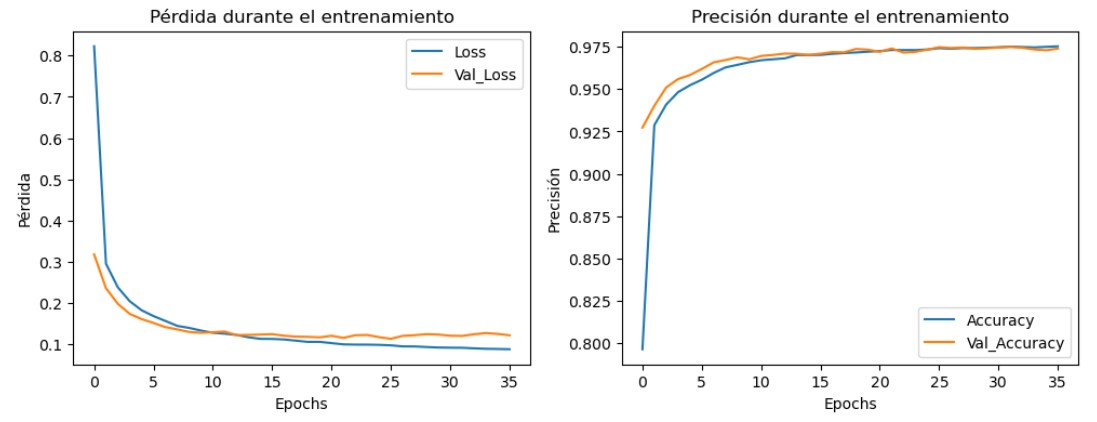
\includegraphics[width=\textwidth]{img/Gráfico modelo clasificación.jpg}        
    \end{minipage}

    \begin{minipage}[t]{0.9\textwidth}
        Fuente: Elaboración propia.
    \end{minipage}
\end{figure}

\subsection{Predicción del modelo}

En la aplicación de nuestro modelo de clasificación secuencial para la generación de predicciones, se procesa una secuencia de acciones previas ejecutadas por un usuario. El modelo utiliza este historial para inferir cuál podría ser la siguiente acción del usuario. Un aspecto distintivo de este modelo es su capacidad no solo para identificar la acción subsiguiente más probable, sino también para cuantificar la confianza en dicha predicción, expresándola en términos de probabilidad.

Por ejemplo, consideremos un caso donde el historial de un usuario indica que está en proceso de recolección de información. Si el modelo anticipa que la acción siguiente será \texttt{getDetails()}, esta predicción se acompaña de una probabilidad asignada, por ejemplo, del 95\%. Tal porcentaje refleja la confianza del modelo en que \texttt{getDetails()} será la próxima acción del usuario. Esta métrica de confianza es fundamental para interpretar no solo las expectativas del modelo sobre eventos futuros, sino también el nivel de certeza asociado a estas expectativas.

En un escenario diferente, si un usuario ha estado interactuando con su cuenta y el modelo pronostica que la acción siguiente será \texttt{getSSContributionsCertificate()}, esta predicción puede presentar una probabilidad del 78.76\%. Este valor sugiere que, aunque el modelo se inclina por \texttt{getSSContributionsCertificate} como la acción probable, existe una notable incertidumbre, posiblemente atribuible a la variabilidad en el comportamiento del usuario o a patrones ambiguos en sus acciones anteriores.

Estos ejemplos demuestran cómo el modelo va más allá de la toma de decisiones binarias, proporcionando un marco cuantitativo que resulta invaluable para la toma de decisiones basada en datos. Este enfoque permite a los sistemas automatizados o a los operadores humanos comprender con mayor profundidad y responder de manera más efectiva a las predicciones generadas por el modelo.
\subsection{Métricas de predicción aplicadas}

Explicaremos a continuación las métricas utilizadas para evaluar el rendimiento del modelo de clasificación, detallando también los resultados obtenidos y su interpretación:

\subsubsection{Precisión (Precision)}
La precisión constituye una métrica crítica en la evaluación de modelos de clasificación. Esta métrica proporciona una estimación de la fiabilidad de las predicciones positivas generadas por el modelo. En términos más concretos, la precisión representa el porcentaje de instancias clasificadas correctamente como positivas por el modelo, en relación con el total de instancias que el modelo ha identificado como positivas, particularmente en escenarios de clasificación multiclase.

Al referirse a una precisión del 57.94\% (o 0.5794 en formato decimal), se está indicando que, bajo las condiciones actuales de modelado, existe una probabilidad del 57.94\% de que una instancia clasificada por el modelo en una categoría específica sea una clasificación acertada. Esta interpretación de la precisión es crucial para comprender la eficacia del modelo en la identificación correcta de las categorías relevantes.

\subsubsection{Recall (Sensibilidad o Tasa de Verdaderos Positivos)}
El \textit{recall} es una medida que indica qué proporción de instancias realmente positivas han sido identificadas correctamente por el modelo. Es decir, del total de instancias que verdaderamente pertenecen a una clase, el \textit{recall} muestra qué porcentaje ha sido reconocido de forma acertada por el modelo.

Con un \textit{recall} de 0.5487 (o 54.87\%), esto sugiere que el modelo logra identificar correctamente el 54.87\% de todas las instancias positivas presentes en el conjunto de datos.

\subsubsection{Puntuación F1}

La puntuación F1 constituye una métrica integral en la evaluación del rendimiento de un modelo de clasificación. Esta métrica es particularmente relevante cuando se busca un equilibrio entre la precisión (precision) y el recall, siendo especialmente útil en contextos donde existe una distribución desigual de clases. Dicho desequilibrio se presenta cuando una clase es significativamente más frecuente que otra.

La puntuación F1 se define como la media armónica de la precisión y el recall. Esta media tiende a favorecer los valores menores dentro del conjunto, lo que implica que un rendimiento alto tanto en precisión como en recall es esencial para alcanzar una puntuación F1 elevada. La puntuación F1 varía entre 0 y 1, donde 1 representa la perfección y 0 la peor puntuación posible.

En el caso de nuestro modelo, con una puntuación F1 de 0.5366 (o 53.66\%), se refleja un equilibrio moderado entre la precisión y el recall. Una puntuación de 53.66\% sugiere un desempeño intermedio, indicando que el modelo no sobresale en ninguna de las dos métricas de manera excepcional, pero tampoco presenta deficiencias significativas. Sin embargo, se preferiría una puntuación F1 más alta, lo que indicaría una mayor armonía y efectividad en el equilibrio entre precisión y recall.

\subsection{Conclusión del Modelo de Predicción Secuencial}

El modelo de predicción de secuencias se ha desarrollado con el propósito de anticipar futuras acciones de usuarios basándose en patrones de comportamiento históricos. Aunque el modelo demuestra una capacidad moderada en la clasificación y predicción de estas acciones, evidenciado por una precisión del 57.94\% y un recall del 54.87\%, los resultados sugieren que existe un margen considerable para mejorar tanto su precisión como su fiabilidad.

La puntuación F1 de 53.66\% refleja un equilibrio entre la precisión y el recall, pero también destaca la necesidad de optimizar el modelo para mejorar su rendimiento predictivo. Esto podría realizarse a través de la refinación de la arquitectura del modelo, la implementación de ajustes en la regularización o la utilización de un conjunto de datos más extenso o representativo.

A pesar de que el modelo actual constituye un punto de partida robusto para la predicción de comportamientos futuros basándose en datos históricos, es claro que para aplicaciones que requieren alta precisión o son críticas, se hace imprescindible una optimización y evaluación adicional. Este proceso de análisis y mejora continua es crucial, particularmente en contextos donde los errores en la predicción podrían tener implicaciones significativas.

Por lo tanto, aunque el modelo actual no alcanza aún los estándares requeridos para una predicción altamente precisa y confiable, representa un avance significativo hacia el entendimiento y la anticipación del comportamiento del usuario. La estrategia a futuro se centrará en la mejora y ajuste del modelo existente, así como en la exploración de nuevas técnicas y metodologías que se alineen más efectivamente con los objetivos de predicción del comportamiento.